\documentclass[12pt]{article}

\usepackage{sbc-template}
\usepackage{graphicx,url}
\usepackage[utf8]{inputenc}
\usepackage[brazil]{babel}
\usepackage[utf8]{inputenc}  
\usepackage{xcolor}
\usepackage{hyperref}
     
\sloppy

\title{Um Mapeamento Sistemático sobre \\Métodos de Identificação Preditiva de Alunos com \\Risco de Reprovação em Educação de Computação}


\author{Lucas R. Costa \and Caique L. Souza \and
\\Ana Carolina G. Inocêncio \and Esdras L. Bispo Jr.}


\address{Instituto de Ciências Exatas -- Universidade Federal de Jataí (UFJ)\\
  75800-000 -- Jataí -- GO -- Brasil
  \email{lucas.costa67@yahoo.com.br, bispojr@ufg.br}
}

 %\textbf{Palavras-chaves}: Educação de Computação, Previsão, Inteligência Artificial, %\textit{Peer Instruction}, Redes Neurais Artificiais.

\begin{document} 
%lucas.costa67@yahoo.com.br, caique12\_@hotmail.com, \{anacarolina.inocencio, esdraspiano\}@gmail.com
\maketitle

\begin{abstract}
  [TRADUZIR]
  This mapping is intended to highlight the difficulties of estimating the final performance of students in the course of Computer Science, after the beginning of the course, as well as methods proposed for this. In total, 81 papers were found. In applying the inclusion and exclusion criteria, 33 papers were selected for a thorough reading, which led to the choice of 18 (?) articles for this article. With the mapping, it was realized that it is possible to predict, with a certain level of precision, the students with risk of reprovation and that avoiding these, reduces the chance of evasion to these students of the course.
  [TRADUZIR]
\end{abstract}
     
\begin{resumo} 
Este mapeamento tem a intenção de elencar as dificuldades de se estimar o desempenho final dos alunos do curso de Ciência da Computação, ainda no início da disciplina, bem como métodos propostos para tal. No total, foram encontrados 81 trabalhos. Ao aplicar os critérios de inclusão e exclusão foram selecionados 33 trabalhos para uma leitura minuciosa, o que levou a escolha de 12 (??) artigos para este artigo. Com o mapeamento, percebeu-se que é possível prever, com certo nível de precisão, os alunos com risco de reprovação e que evitando estas, diminui-se a chance de evasão destes alunos do curso.
\end{resumo}


\section{Introdução}

Um excelente ponto de partida para descrever a Pesquisa em Educação de Computação (PEC) são as duas áreas de sua junção: a Educação e a Ciência da Computação. Pode-se definir, como um dos objetivos principais da PEC, o aperfeiçoamento do processo de ensino e aprendizagem da Computação como ciência \cite{holmboe:2001}. Existem muitos desafios abertos na PEC \cite{robins:2015}. Um deles está associado ao alto índice de evasão registrado em cursos superiores de Computação.

A aprendizagem da Computação, como Ciência, pode apresentar dificuldades para o aprendiz iniciante, assim como outras áreas de exatas \cite{Blando2015}. Segundo dados do Censo da Educação Superior de 2017 \cite{Inep2017}, publicado pelo Instituto Nacional de Estudos e Pesquisas Educacionais Anísio Teixeira (Inep) do Ministério da Educação (MEC), a taxa de evasão do Bacharelado em Ciência da Computação alcançou cerca de 60,2\%, enquanto a taxa geral ficou em torno dos 26\%, mostrando que o problema está se agravando no curso.

Muitas vezes os ingressantes não conseguem acompanhar o fluxo de estudos, têm baixo desempenho e assim acabam evadindo ou reprovando nas matérias introdutórias do curso. Com taxas de evasão tão altas, um dos desafios constantes da PEC é identificação prévia de estudantes em risco de reprovação ou evasão \cite{Porter2014}. Muitos métodos de identificação foram apresentados, como o modelo de ARL(Análise de Regressão Linear) usando os dados coletados utilizando o IpC(Instrução pelos Colegas) para previsão do desempenho do exame final \cite{Liao2016}, como o modelo PreSS que pode auxiliar na identificação do alunos em risco \cite{Quille2018}, e ate ferramentas capazes de tirarem \textit{snapshots} dos código-fonte auxiliando na identificação das dificuldades apresentadas pelos alunos usando aprendizado de máquina \cite{Ahadi2016a}. Entretanto, ainda existe uma lacuna no que diz respeito a trabalhos secundários na área, como por exemplo, mapeamento sistemático.

%Tema
Este trabalho tem como propósito realizar um mapeamento sistemático sobre os métodos de identificação preditiva de alunos com risco de reprovação em Educação de Computação. O objetivo deste mapeamento é possibilitar pesquisadores a identificar os principais métodos, contrastando-os entre si ou com novos métodos a serem propostos. Além disso, este mapeamento permitirá que novas pesquisas provejam para o professor ou gestor educacional um leque de ferramentas que os auxiliem na tomada de decisão em vistas à ações político-pedagógicas que enfrentem o problema do alto índice de reprovação e de possíveis casos futuros de evasão.

O restante do trabalho é dividido como se segue. A Seção \ref{sec:metodologia} apresenta a descrição metodológica do como foi realizado o mapeamento sistemático. A Seção XXX... A Seção xXX. E, por fim, as considerações finais (Seção \ref{sec:consideracoes}) são apresentadas.


\section{Metodologia} \label{sec:metodologia}

\subsection{Descrição do Problema}
Como identificar alunos em situação de risco de reprovação em uma disciplina na Ciência da Computação?

\subsection{Objetivo}
O objetivo deste Mapeamento Sistemático é fazer uma revisão, seleção e organização dos artigos que possam identificar os alunos em situação de risco, analisando os métodos utilizados pelos outros autores para solucionar o problema supracitado.

\subsection{Questões de Pesquisa}
Para nortear esta pesquisa, foram definidas questões que levantem pontos relevantes a serem estudados.

\begin{itemize}
    \item \textbf{Questão 1:} Quais métodos existem para identificar risco de reprovação em disciplinas?
    \item \textbf{Questão 2:} Quais os indícios de que um aluno pode ser reprovado, baseado em dados gerados pela avaliação formativa?
    \item \textbf{Questão 3:} Quais as medidas que existem para impedir esta reprovação?
\end{itemize}

\subsection{Palavras-chave e strings de busca}
As palavras-chave que compõem a busca são (em português e inglês, respectivamente): Educação de Computação, Ensino de Computação, Introdução a Computação, Avaliação, Estimativa, Previsão, Inteligência Artificial, Mineração de Dados, Aprendizado em Profundidade, Redes Neurais Artificiais, RNA, \textit{Computer Education}, \textit{CS1}, \textit{Assessment}, \textit{Prediction}, \textit{Artificial Intelligence}, \textit{Data Mining}, \textit{Clicker}, \textit{Deep Learning}, \textit{Artificial Neural Network}, \textit{ANN}.

A string de busca foi gerada a partir da combinação das palavras chave e foram divididas pelos idiomas da seguinte forma: 

    \textit{\textbf{Português}}: ("Educação de computação" OR "ensino de computação" AND "Introdução a Computação" OR “Avaliação”) AND ("estimativa" OR "previsão" OR "Inteligência Artificial" OR "mineração de dados" OR “Clicker”OR “Aprendizado em Profundidade” OR "Redes neurais" OR “RNA”)

    \textit{\textbf{Inglês}}: ("computer education" AND "cs1" OR "assessment") AND ("prediction" OR "data mining" OR "artificial intelligence" OR "clicker" OR "deep learning" OR "Artificial neural network" OR "ANN"))

\subsection{Método utilizado para pesquisa}
Os seguintes critérios de inclusão foram definidos e aplicados na seleção dos trabalhos relevantes: O trabalho deve estar escrito em inglês ou português; a versão completa do trabalho estar disponível na internet; apresentar necessidade de identificar os alunos em situação de riscos;  apresentar os métodos utilizados para identificar esses alunos. Os Critérios de Exclusão utilizados foram: não possuir a versão completa disponível na internet; não apresentar os métodos de identificação dos alunos em risco de reprovação; não apresentar a necessidade de identificação de alunos em situação de risco; verificar trabalhos que são réplicas, priorizando o trabalho mais recente.

Aplicou-se o método de pesquisa preestabelecido para a identificação de potenciais trabalhos relacionados ao tema deste mapeamento. 
As máquinas de busca utilizadas para a pesquisa foram: \textit{ACM Digital Library} (https://dl.acm.org/) e \textit{Google Scholar} (https://scholar.google.com.br).
Os idiomas definidos para busca e seleção dos artigos foram português e inglês, no período de 2013 a 2018. Foram recuperados, no total, 67 trabalhos em inglês e 14 em em português.

Foi realizada uma triagem, que consistiu na leitura do título, do resumo/\textit{abstract} e das palavras-chave/\textit{keywords} dos trabalhos previamente recuperados, aplicando os critérios de inclusão e exclusão. 
33 trabalhos foram pré-selecionados; 3 dos 48 trabalhos rejeitados, se tratavam apenas do \textit{abstract}. 
A maioria foi rejeitada, pois os trabalhos não apresentavam métodos, para identificar os alunos com possibilidade de reprovação e muitos deles tratavam apenas de métodos de ensino e ferramentas, para auxílio do ensino.
A partir do conjunto preliminar de trabalhos, realizou-se uma leitura minuciosa dos textos completos dos mesmos. Nesta etapa, os critérios de inclusão e exclusão foram reaplicados. 
Dos 33 trabalhos selecionados, 18 (??) trabalhos foram escolhidos. A maioria foi rejeitada pois os trabalhos não apresentavam a necessidade de identificar os alunos em situação de riscos e, consequentemente, não apresentavam métodos para tal.

\section{Resultados e Discussões}

Ao ler os artigos selecionados, foram encontrados diversos métodos na tentativa de identificar os alunos com risco de reprovação, e a maioria dos métodos encontrados utilizavam técnicas estatísticas na análise dos dados.

Outros trabalhos utilizaram como técnica preditiva a aprendizagem de máquina e outras técnicas de Inteligência Artificial. Nesta seção será apresentado uma discussão em torno das questões estabelecidas para nortear o artigo.

Na primeira questão será apresentado as técnicas preditivas usadas nos trabalhos correlatos selecionados no mapeamento. A segunda questão trata dos indícios de reprovação que podem ser encontrados na avaliação do aluno. E, por fim, a terceira questão traz a tona a discussão, o que pode ser feito para evitar estas situações.

\subsection{\textbf{Questão 1: Quais métodos existem para identificar risco de reprovação em disciplinas?}}


 A tabela a seguir apresenta a relação dos artigos estudados neste mapeamento e os métodos utilizados por cada um, na tentativa de predição de desempenho dos alunos. A tabela apresenta a quantidade de artigos que utilizaram cada método.

\begin{figure}[ht]
\centering
\caption{Métodos utilizados por cada artigo}
\label{tab:exTable1}
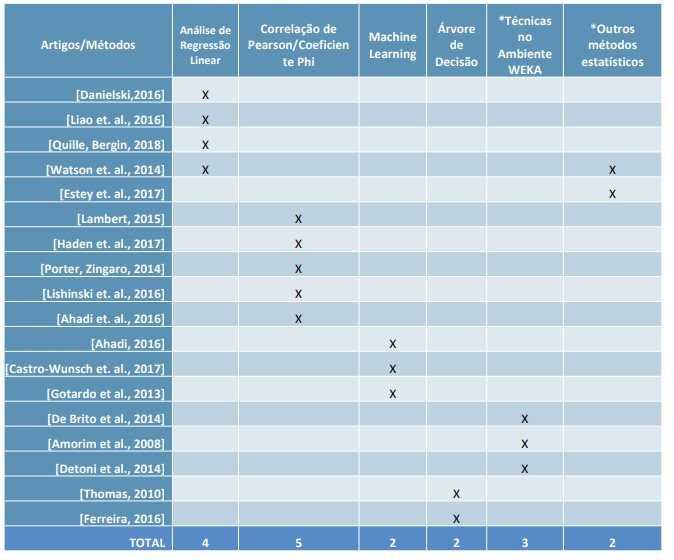
\includegraphics[width=1\textwidth]{Taable.jpg}
\label{fig:table}
\subcaption{* = Shapiro-Wilks e Métricas de Trajetória e de Linha de Base}
\end{figure}


%\begin{table}[h]
%\centering
%\caption{Métodos utilizados}
%\vspace{0.5cm}
%\begin{tabular}{|r|l|}
%\hline
%Métodos                                & Total de Artigos\\ \hline
%Métricas de Trajetória e Linha de Base & 1     \\ \hline
%Correlação de Pearson/Coeficiente Phi  & 5     \\ \hline
%Análise de Regressão Linear            & 4     \\  \hline
%Shapiro-Wilk Test                      & 1     \\   \hline
%Machne Learning                        & 2     \\\hline
%\end{tabular}
%\end{table}

No trabalho realizado por Liao et. al.\cite{Liao2016}, os dados foram extraídos ao utilizar o método IpC (Instrução pelos colegas) e, com esses dados, construiu-se um \textbf{Modelo de ARL} para examiná-los, o qual criado através dos principais componentes, escolhido pelo PCA (\textit{Principal Component Analysis}), prevendo a nota que seria obtida no exame final. Outros autores que utilizaram o IpC, na coleta de dados, foram Porter e Zingaro \cite{Porter2014}, porém eles utilizaram a \textbf{CPMP (Correlação de Produto-Momento de Pearson)} para analisar os dados, e assim verificar o quão relacionado está o desempenho do aluno ao decorrer do curso com o sucesso obtido no final do mesmo, e concluiu-se que há correlação entre o resultado obtido entre a 3ª e a 4ª semana com o resultado final do aluno.

No trabalho de Lishinski et. al.\cite{Lishinski2016}, foram utilizadas tarefas de múltipla escolha, em que cada item possuía ponderações diferentes, para medir a capacidade dos alunos na resolução de problemas, podendo assim calcular a CPMP entre os resultados obtidos em aula e o resultado final. Usando uma abordagem mais ampla, Lambert \cite{Lambert2015}, também faz a CPMP, porém com alguns fatores que podem levar o aluno a reprovação, entre eles, a capacidade matemática e o conhecimento prévio em programação. Haden et. al. \cite{Haden2017} usaram a CPMP para que se possa medir a afetividade do aluno em relação ao ambiente e a influência no resultado obtido no CS1 (\textit{Computer Science 1} - Introdução). Outro trabalho a utilizar a CPMP, em conjunto com a \textbf{Coeficiente Phi}, foi o de Ahadi, Lister e Vihavainen \cite{Ahadi2016} que, conseguiram identificar relações existentes entre o número de tentativas na resolução dos problemas de programação e o resultado final obtido. 

O trabalho do Danielsiek \cite{Danielsiek2016}, após a extração dos dados, faz a ARL e verifica a relação entre os resultados obtidos durante as aulas e os resultados finais da disciplina. Fazendo uma ARL mesclada ao teste de normalidade \textbf{Shapiro-Wilks}, Watson, Li e Godwin \cite{Watson2014} testaram o quão preditor um conjunto de 50 variáveis pode ser, ao tentar identificar os alunos em situação de risco de reprovação, mostrando qual variável tem maior desempenho em predizer o resultado final do aluno. Já o trabalho de Quille e Bergin \cite{Quille2018} apresenta o \textbf{Modelo PreSS}, criado há 20 anos, que teria a capacidade de identificar os alunos em situação de risco de reprovação, modelo esse que faz a análise de regressão dos dados.

Alguns trabalhos utilizaram outros métodos como, por exemplo, \textbf{Aprendizado de Máquina}. Ahadi \cite{Ahadi2016a}, que faz uso de uma ferramenta capaz de capturar \textit{snapshots} dos códigos-fonte produzidos pelos alunos, em um curso introdutório de programação, faz o uso do aprendizado de máquina para identificar os alunos com dificuldade. Já o trabalho de Castro-Wunsch, Ahadi e Petersen \cite{Castro-Wunsch2017}, com o auxílio de uma Rede Neural Artificial (RNA), identifica os alunos que estão em risco de reprovação. Estey, Keuning e Coady \cite{Estey2017} utilizam uma ferramenta que coleta o número de submissões feitas e a quantidade de dicas usadas pelos alunos para que o modelo criado possa realizar o cálculo das \textbf{Métricas de Trajetória e de Linha de Base} para a identificação dos alunos que necessitam de auxílio.

Outro trabalho que apresenta uma abordagem usando algoritmos de aprendizado máquinas, foi o de Gotardo et. al. \cite{Gotardo2013}. Os algoritmos foram acoplados para integrar diferentes técnicas de aprendizado e mineração de dados e explorar um conjunto de dados educacionais. Os algoritmos foram: NaiveBayes e J48.

Alguns trabalhos utilizaram, como técnica de identificação de alunos em situação de risco de reprovação, a \textbf{Árvore de Decisão}. Um destes é o de
H. Thomas \cite{Thomas2010} objetifica-se a propor um algoritmo - usando a técnica de árvore de decisão - que identifique os alunos em risco e gere relatórios para acompanhamento, ao usar a plataforma de ensino \textit{Moodle}. O trabalho demonstrou uma precisão de 72\%.

Outro trabalho que utilizou a árvore de decisão foi o de Ferreira \cite{Ferreira2016}, que propõe um modelo para predição de grupos de risco. A técnica de árvore de decisão foi utilizada para possibilitar um diferencial quanto à possibilidade de interceptação dos dados gerados pelo uso dos métodos de predição, pois outros métodos, como RNA possuem como deficiência justamente a dificuldade de identificar as causas que levam aos resultados das predições.

Alguns trabalhos utilizaram o \textbf{Ambiente WEKA}. O WEKA é um pacote de software que acopla vários algoritmos de Inteligência artificial. Os trabalhos escolhidos que utilizaram a ferramenta, analisaram a atuação de alguns dos principais algoritmos, para a identificação de grupos de risco.

Um destes trabalhos foi o realizado por Daniel et. el. \cite{DeBrito2014}. O trabalho visa identificar os alunos que necessitam de apoio didático no início do curso, Ao usar a Mineração de Dados Educacionais, para evitar a evasão do curso. 
O trabalho avalia a relação entre as notas de ingresso do aluno e o seu desempenho no primeiro período do curso. Os algoritmos foram: Nayve Bayes, IBk, SMO, Random Florest e Multi Perceptron. O trabalho obteve precisão superior a 70\%.

Outro trabalho ao utilizar o WEKA foi o de Maurício et. al. \cite{Amorim2008}. O artigo demonstra as principais fases para implementação de um sistema de previsão testa a acurácia de três classificadores amplamente utilizados e mostra as estatísticas referentes a evasão em cada curso. Foram usados: Redes Bayesianas, SMO e J48, os 3 principais algoritmos do WEKA.

E, por fim, o trabalho de Detoni \cite{Detoni2014}, objetifica-se a desenvolver e testar técnicas e modelos de aprendizagem de máquina no ambiente Moodle. Modelos gerados e avaliados uando WEKA: Rede Bayesiana, Rede Neural, J48 e Random Florest.
a acurácia média alcançada foi superior a 90\%. A precisão ficou entre 75\% e 95\%.


\subsection{\textbf{Questão 2: Quais os indícios de que um aluno pode ser reprovado, baseado em dados gerados pela avaliação formativa? }}


A possibilidade de reprovação pode ser prognosticada através de variáveis preditivas, e com estes indícios descritos, pode-se dar ao professor a possibilidade de readequar sua metodologia e traçar novas estratégias de ensino para que possa evitar tais reprovações. Liao et. al.\cite{Liao2016}, com os dados obtidos, criaram um modelo capaz de classificar os alunos e identificar a situação destes, com uma precisão de 70\%, utilizando os dados de testes e treinamentos das 3 primeiras semanas.

O framework PISA, utilizado por Lishinski et. al.\cite{Lishinski2016}, possibilita medir a capacidade do aluno de resolução de problemas, sendo parte essencial do aprendizado de programação. Ele deixa claro que a programação é um conhecimento hierárquico, onde cada conteúdo assimilado serve de base para os posteriores. De forma semelhante, Ahadi \cite{Ahadi2016a} coleta os dados com uma ferramenta capaz de capturar \textit{snapshots} dos códigos-fonte gerados, podendo apresentar ao professor as dificuldades dos alunos. Castro-Wunsch, Ahadi e Petersen \cite{Castro-Wunsch2017} demonstraram que os dados obtidos, processados por uma Rede Neural, obtêm um bom resultado na predição do sucesso dos alunos, com resultado de 80-85\% de variação em sua eficiência. %[? Haden et. al.\cite{Haden2017} apresentaram uma ferramenta construída para o seu trabalho, e que os dados fornecidos para o professor podem ser utilizados para encontrar aluno em situação de risco. Outros autores que utilizam ambiente online são Ahadi, Lister e Vihavainen \cite{Ahadi2016}, e muitos dos trabalhos utilizando ambiente de programação possui características semelhantes ?]. 
Estey, Keuning e Coady \cite{Estey2017} apresentam uma ferramenta com o diferencial de apresentar um \textit{feedback} para o aluno, assim, além do professor, o aluno também pode saber como está sua compreensão em relação aos conteúdos.

Algumas variáveis preditoras, exploradas por Lambert \cite{Lambert2015}, são: o histórico acadêmico do aluno, fatores matemáticos e experiências anteriores dos alunos, porém ele só encontrou uma correlação forte com o CS0 (\textit{Computer Science 0} – Curso Prévio) no sucesso do CS1, enquanto não teve sucesso com as demais variáveis utilizadas. No trabalho de Watson, Li e Godwin \cite{Watson2014}, é feito um teste de 50 diferentes preditores de desempenho, sendo 38 tradicionais e 12 dinâmicos, ambos baseados no comportamento de programação, tendo uma maior eficácia nos cursos de CS1.

Através de um ambiente de virtual de Marques, Andrade e Tessari \cite{} mostra-se que os dados gerados na plataforma Moodle, utilizando o seu algoritmo proposto são excelentes variáveis proditoras tendo uma precisão de 72\%, mostrando assim o desempenho da utilização de ambiente virtuais no ensino e a capacidade preditiva da árvore de decisão. Usando também o ambiente virtual Detoni, Moodle, Araujo e Cechinel \cite{Detoni2014}, e a partir dos dados gerados pelo alunos foi gerado modelos dos quais foram avaliados pelo WEKA, assim utilizando vários algoritmos de inteligência artificial como Rede Bayesiana, Rede Neura, J48 e Random Florest, apresentados os resultados obtidos dos mesmos tendo umas media de acurácia superior a 90\% e com uma precisão entre 75\% e 95\%. Brito, Daniel e Araújo \cite{DeBrito2014} utiliza-se de dados educacionais para apresentar uma abordagem que usa algoritmos de aprendizagem acoplados para integrar diversos técnicas de aprendizado e mineração de dados, tais algoritmos como NaiveBayes e J48, mostrando mais um pouco a relevância do algoritmo de inteligência artificial como ferramenta no ensino. 

Gotardo et al. \cite{Gotardo2013} avalia a relação entre as notas notas de ingresso do aluno com seu desempenho ao decorrer do curso, utilizando os algoritmos presentes na ferramenta WEKA tais como Nayve Bayes, IBk, SMO, Random Forest e Multi Perceptron, e obteve um resultado superior a 70\% com essa ferramenta, podendo se notar a relação entre as notas de ingresso e as notas ao decorrer do primeiro período de curso. Amorim, Barone e Mansur \cite{Amorim2008} mostra-se as principais fases na implementação de um sistema de previsão e fez o teste de três classificadores amplamente utilizados e mostra as estatísticas referentes a evasão em cada curso, e demonstra a eficácia das técnicas de Machine Learning presentes na ferramenta WEKA. Ferreira, Barbosa e Rigo \cite{Ferreira2016} propõe um modelo para predição de grupos de risco com técnicas de árvore de decisão, e obteve resultados mostrando a possibilidade de interceptação dos dados gerados pelo uso dos métodos de predição, pois métodos, como RNA possuem como deficiência justamente a dificuldade de identificar as causas que levam aos resultados das predições.

\subsection{\textbf{Questão 3: Quais as formas que existem para impedir esta reprovação?}}
As formas existentes para impedir a reprovação do aluno são unanimemente abordadas da mesma forma nos artigos, pois o objetivo é predizer o resultado dos alunos durante alguma disciplina no curso de Ciência da Computação, ao detectar padrões que auxiliem o processo de classificação destes alunos em grupos com desempenhos semelhantes. Estas formas servem para que os professores possam criar uma estratégia para realocar os fatores da disciplina, baseado nos resultados obtidos para disseminar de forma clara e consistente, todos os fundamentos necessários para formação de um bom profissional. O professor, tendo em mãos a relação dos alunos que possuem possibilidade de reprovação, pode reorganizar a forma que ministra sua aula, oferecer auxílio-extra aos alunos, ou qualquer outra estratégia para evitar estas reprovações.

\section{Considerações Finais} \label{sec:consideracoes}

O mapeamento sistemático teve como foco os métodos para identificação de aluno em situação de risco de reprovação e a correlação entre os resultados obtidos no período inicial da disciplina com a nota final do exame. As questões de pesquisa foram criadas com o intuito de descobrir quais métodos foram utilizados pelos principais autores na área e a eficácia destes. 

A questão 1 mostra vários métodos na identificação de alunos com possibilidade de reprovação, concluindo que os mais eficientes para tal são os métodos de estatística descritiva, dentre eles o mais eficaz e mais utilizado é o método de Correlação Produto-Momento de Pearson. A questão 2 analisa os possíveis indícios de reprovação apresentados durante o período do curso, concluindo-se que, a partir da classificação obtida através dos métodos apresentados para a análise dos dados gerados, poderia se prever o desempenho final dos alunos. A questão 3 analisa as formas de impedir a reprovação, já que através dos métodos avaliados neste artigo, o professor teria em mãos, dados necessários para traçar novas estratégias de ensino.

Esta pesquisa teve por objetivo o levantamento de métodos que prevejam o desempenho final dos alunos, para que uma intervenção seja feita, a fim de evitar eventuais reprovações. Um ponto importante, que foi possível observar com este mapeamento, é que métodos estatísticos descritivos alcançam níveis preditivos expressivamente altos. 

\bibliographystyle{sbc}
\bibliography{sbc-template}

\end{document}
